\section{Join Ordering}
Join ordering focuses on conjunctive queries with simple predicates of the type $a_1 = a_2$ where the latter can be either an attribute or a constant (commonly algorithms assume join between attributes).

Relations may include selections or complex building blocks, however for simplicity filtering is ignored; having operators other than equality might cause differences within the query planner.

Ordering basically means choosing which relation to be joined first, placing entities in a graph and adding an edge whenever a predicate from a node is joined to another. 

This kind of schema is defined as a query graph, in which edges consist in predicates and self loops represent equality with a constant. Usually cycles are pushed down, since algorithms only assume attributes. 

Based on the query graph it is possible to obtain an overview of the complexity of the problem: there are different shapes which are treated differently. 

\begin{figure}[h]
	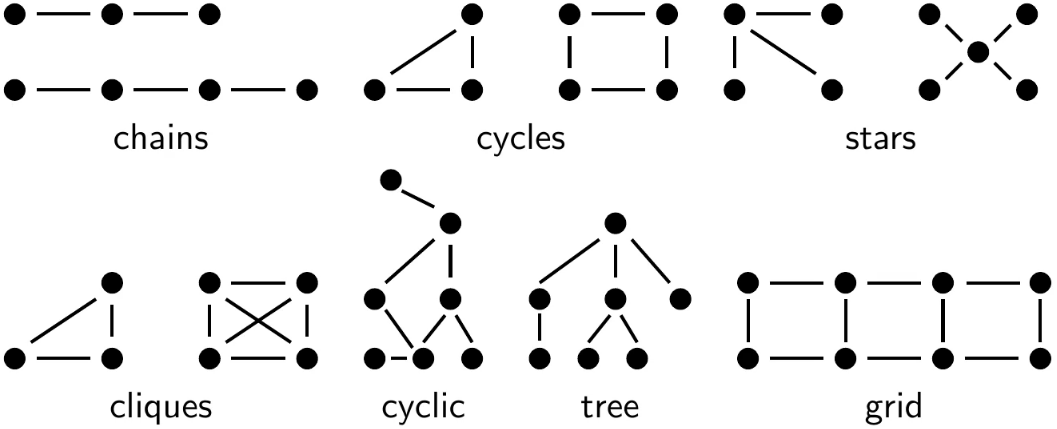
\includegraphics[scale=1.5]{query_graph.png}
	\centering
\end{figure}

\begin{enumerate}
	\item Chains are the simplest kind of query, fairly common in practice;
	\item Cycles (cyclic) are a chain with a closing edge, the easiest example of cycles;
	\item Stars are mostly used in data warehouse, in which the center table has large dimension and the ones outside are relatively small, quite different to solve;
	\item Cliques are instances in which every relation is joined with all the others, and are the hardest to optimize causing the worst runtime;
	\item Trees are acyclic queries even if the level of nesting can be high;
	\item Grids are also fairly hard and interesting for research.
\end{enumerate}

Joins are represented with join trees, binary trees with operators as inner nodes and relations as leaves. The most common type is unordered (not distinguish left from right) without cross product, however algorithms might produce other variants.

There furthermore are different kinds of trees:
\begin{itemize}
	\item Left-deep tree, in which joins only happen on the left side, easy to represent and implement through hash tables ($n!$ trees with cross products);
	\item Right-deep tree ($n!$);
	\item Zig-zag tree, a combination of the previous ($n!2^{n-2}$);
	\item Bushy tree, a full binary tree (non-linear, harder to find optimal solutions but can be the most efficient in some cases, $n!C(n-1) = \frac{(2n-2)!}{(n-1)!}$ where $C$ represents a Catalan number).
\end{itemize}
It is relevant to notice that the number of leaf combinations and unlabeled trees grows exponentially, and increases even more with a flexible structure. However, nodes can often be swapped from left to right.

Another important information about joins is their selectivity: 
$$f_{i, j} = \frac{\abs{R_i \bowtie_{p_{i, j}} R_j}}{\abs{R_i \times R_j}}$$
This depends on whether the attributes are a key, and gives an estimation of the result cardinality with the aid of assumptions and statistics.

Given a join tree, the cardinality can be computed recursively as the productory of the selectivity function multiplied by the size of both relations. This allows easy calculations only requiring base cardinalities and independence of predicates:
$$C_{out}(T) = \begin{cases}
0 & T\text{ is a leaf} \\
\abs{T} + C_{out}(T_1) + C_{out}(T_2) & T = T_1 \bowtie T_2
\end{cases}$$
This formula sums up the sizes of intermediate results, which are the ones causing more works. There are basic specific cost functions for joins, to be summed to the cost of single relations. 

Algorithms are mainly designed for left-deep trees, and some of the cost functions do not work in practice, for instance in the case of cross products. Therefore, those indicators are mainly theoretical and work under strict assumptions. However, join ordering is a main factor regardless of the chosen cost methods.

A cost function is called symmetric if $C_{impl}(e_1 \bowtie^{impl} e_2) = C_{impl}(e_2 \bowtie^{impl} e_1)$. Commutativity can be ignored.

Most of the time, algorithms for query optimization tend to avoid cross products, despite the enormous number of possibilities to build a join tree: the only exception regards small relations.

\subsubsection{Chains}
Chains usually originate a left-deep tree: leaves can be ordered according to different degrees of freedom, as long as all the relations are joined. 

The number of possible left-deep trees can be defined recursively:
$$\begin{cases}
f(0) = 0 \\
f(1) = 1 \\
f(n) = 1 + \sum_{k=1}^{n-1} f(k-1) \cdot (n - k)
\end{cases}$$
Adding $R_n$ to all possible join trees can be done at any position following $R_{n-1}$. There are $n - k$ join trees for $R_n$, plus one assuming it can be placed before $R_{n-1}$ in the case of $k=1$. For $R_{n-1}$ to be at $k$, $R_{n-k} - \dots R_{n-2}$ must be below it.

Solving the recurrence gives the closed form $f(n) = 2^{n-1}$, still exponential yet much less than the case with cross products.

A generalization to zig-zag can be made expecting the same result.

Bushy trees, on the other hand, are not so easy to obtain: each subtree must contain a subchain to avoid cross products, hence single relations should not be added. It is possible to create a whole chain $R_1 - \dots R_n$, cut it and place it under another subtree, always considering commutativity.

This gives the formula:
$$ f(n) = \begin{cases}
1 & n < 2 \\
\sum_{k=1}^{n-1} 2f(k) \cdot f(n-k) & n \geq 2
\end{cases}$$
Having more than 2 relations implying performing a cut at some point $k$ and placing $k$ on the left side, $n - k$ on the right side. A factor of 2 indicates swapping the two sides. 

This gives the closed form $f(n) = 2^{n-1}C(n-1)$.

\subsubsection{Stars}
Star queries have the constraint that one relation must be in the center; all the others can be ordered arbitrarily. This leads to the following formulas:
\begin{itemize}
	\item Left-deep: $2 \cdot (n - 1)!$, since there are $n - 1$ choices for a join partner and a factor of 2 for commutativity;
	\item Zig-zag: $2 \cdot (n - 1)! \cdot 2^{n-2}$, in which the last factor represent the possibility to swap left and right for each subtree;
	\item Bushy trees: not possible since they require the first relation to be available. 
\end{itemize}

\subsubsection{Cliques}
Cliques are a schema which do not care about cross products, since every relation is connected to the other, hence the number of possibilities is the same as the one obtained allowing cross products. 

Still, complexity is very high and runtime is bad, although the worst case usually does not happen. 

\subsection{Greedy heuristics}
Regardless of the methods and the inclusion of cross products, the search space is in general quite large when the number of relations is larger than 10, and polynomial time is hard to achieve. Some cost functions do not even have a proof of complexity.

Due to the size of the search space, greedy heuristics are ways to easily construct a potential tree in a fast time: they are most suitable for large queries, but often do not give the best result.

Algorithms assume no cross products within left-deep trees, and known cardinalities (or some other weight function).

\subsubsection{GreedyJoinOrdering-1}
This algorithm returns a set of ordered relations to be joined according to a cost function in a bushy tree structure. 

The output is given starting from the minimum-weight relation, removes it and searches for the new minimum. 

This method is simple, but not that good in practice: it assumed fixed weight (not depending on the size, for instance) and does not support optimization within intermediate results. 

\subsubsection{GreedyJoinOrdering-2}
This variant also considers the previous set of relations, computing relative weights based on the existing tree. 

In this case, however, the very first relation has a large relative weight and a major impact on the choices made afterwards. 

\subsubsection{GreedyJoinOrdering-3}
To tackle this problem, a double loop is introduced in which not only the set of relations is scanned, but also every relation is tested as a starting one. Then, all computed results are compared and the minimum among them is returned. 

This method is overall the best one and is implemented in some systems, but it is still not optimal.

\subsubsection{Greedy Operator Ordering}
Intermediate join trees must be combined to obtain larger trees: since some algorithms construct left-deep structures and others return bushy trees, those can be attached if the result is minimal: trees with the smallest weight are iteratively joined and then removed by the set of possibilities. 

First, each combination of weight (for instance, product of cardinalities and selectivity) is calculated; then the minimum is chosen and the two relations are aggregated. 

In case both relations are linked to the same (different) one in the query graph, the selectivity of the new edge consists in the product of previous ones. 

This algorithm has two pitfalls: one is its computational complexity of $O(n^3)$, which however can be in the order of milliseconds with small input, and the other is its sub-optimal output in some cases.

In fact, it is not guaranteed that Greedy Operator Ordering finds the best bushy tree given a set of relation, even if it tends to have better results than the greedy ordering techniques.

\subsection{IKKBZ}
IKKBZ is a polynomial time algorithm for join ordering without cross products, producing left-deep trees under some assumptions: acyclic graphs, ASI cost functions and a fixed join technique.

The algorithm will ultimately compute a rank for each predicate, based on its selectivity, obtaining an optimal evaluation order. After the first steps, however, the remaining arguments are independent on the size of the relations.

It starts considering a cost function as a product of the form:
$$C(T_i \bowtie R_j) = \abs{T_i} \cdot h_j(\abs{R_j})$$
Each relation $R$ can have its own $h$, which has a set of parametrized cost functions. Cardinalities are also taken into account, defining $n_i = \abs{R_i}$ and $h_i(n_i)$ as the cost per input tuple of a join. $T_i$ is the left side of the computation.

A predecende graph helps identifying which relations should be joined first; it is represented as an oriented query graph, and constructed with root in $R_k$ in the following way:
\begin{enumerate}
	\item The root is fixed, removed by the set of possibilities and added to the tree;
	\item As long as there are relations to be chosen, $R_i \in V \setminus V_k^P$ is selected such that $\exists\ R_j \in V_k^P : (R_j, R_i) \in E$;
	\item $R_i$ is added to $V_k^P$ and an edge $R_j \rightarrow R_i$ is created.
\end{enumerate}

The algorithm constructs left-deep trees.

A sequence of nodes conforms to a precedence graph if two conditions are satisfied:
\begin{itemize}
	\item For each position $i$, there exists one $j$ coming before;
	\item There does not exist a position $i$ and a $j$ coming after with an edge from $j$ to $i$ (acyclic).
\end{itemize}

If there exists a path between two sets of relations $R_i$ and $R'_i$, all relations from the first must be joined first; there is no join condition between any pair of relations aside from the one joining the two sets, hence the selectivity is 1.

Selectivity of the join:
$$s_i = \begin{cases}
1 & \abs{R_i'} = 0 \\
\prod_{R_j \in R'_i} f_{i, j} & \abs{R'_i} > 0
\end{cases}$$
In case of cycles, the selectivity cannot be uniquely determined: there could be two relations with different values. Therefore, first the precedence graph is fixed, and then selectivities are calculated.

If the query graph is a chain (total order), then the following properties hold:
$$n_{1, 2, \dots, k} = \prod_{i=1}^{k}s_in_i$$
$$C_H(G) = \sum_{i=2}^{n}\big[n_{1, 2, \dots, i-1}h_i(n_i)\big] = \sum_{i=2}^{n}\Big[\Big(\prod_{j=1}^{i}s_jn_j\Big)h_i(n_i)\Big]$$
The cardinality of the joins is equal to the productory of each selectivity for each cardinality among all relations.

If the weight function is indeed the selectivity, then $C_H \equiv C_{out}$. The factor $s_in_i$ determines how much the input relation changes its cardinality before further joins, and can be increasing or decreasing.

The algorithm employs a recursive definition of the cost function:
$$\begin{cases}
C_H(\epsilon) = 0 \\
C_H(R_i) = 0 & \text{the relation is the root} \\
C_H(R_i) = h_i(n_i) & \text{else} \\
C_H(S_1S_2) = C_H(S_1) + T(S_1) \cdot C_H(S_2)
\end{cases}$$
$$T(\epsilon) = 1 \qquad \land \qquad T(S) = \prod_{R_i \in S}s_in_i$$
Last $C_H$ definition corresponds to the cardinality performing all the relation in the sequence (the term $T$) and multiplying for the cost of last element.

This allows to use ASI properties: in fact, these hold if and only if there exists a function $T$ and a rank function defined as:
$$rank(S) = \frac{T(S) - 1}{C(S)}$$
The following must hold:
$$C(AUVB) \leq C(AVUB) \leftrightarrow rank(U) \leq rank(V)$$
In other words, ASI properties hold if and only if the relations can be ordered by rank. The cost function previously defined can be proven to respect these constraints.

It is possible that the rank contradicts the precedence graph: the following definition is introduced to counter this occurrence.

Let $M = \{A_1, \dots, A_n\}$ be a set of sequences of nodes. Then $M$ is called a module if, for all sequences $B$ that do not overlap with the sequences in $M$, one of the following conditions holds:
\begin{itemize}
	\item $B \rightarrow A_i, \forall\ A_i \in M$;
	\item $A_i \rightarrow B, \forall\ A_i \in M$;
	\item $B \nrightarrow A_i \land A_i \nrightarrow B, \forall\ A_i \in M$.
\end{itemize}

If $A \rightarrow B$ and $rank(B) \leq rank(A)$, then it is possible to find an optimal sequence among those in which $B$ directly follows $A$.

The continued process of building a compound relation until no more contradictory sequences exist is called normalization; the opposite is denormalization.

\subsubsection{The algorithm}
IKKBZ works performing the following steps for each relation, considering it as a root node:
\begin{enumerate}
	\item Calculates the precedence graph;
	\item Executes the subprocedure of finding the subtree all of whose children are chains, and normalizing it, then merging the chains;
	\item The relation returned by the previous step is added to the set.
\end{enumerate}
The algorithm stops when all trees are single chains, then returns the minimum of the sets according to the cost function.

The subprocedure constructs a left-deep tree (chain) from the precedence graph, performing a normalization operation and merging based on the rank in ascending order. Normalization happens when there is a contradictory sequence, i. e. one chain has bigger rank than the following.

This works by taking $r$ and $c$ such that $rank(r) > rank(c)$ and swapping them with a compound relation representing both. This allows to merge relations that would have been reordered if only considering the rank, obtaining the actual ascending order.

In case the graph contains cycles, it is possible to preprocess it with algorithms such as Minimum Spanning Tree to find a suitable representation to run IKKBZ.
